\documentclass{article}
\usepackage{graphicx}
\usepackage{multicol}
\usepackage{amsmath}
\usepackage{wasysym}
\usepackage{amssymb}
\usepackage{mathtools}
\usepackage[utf8]{inputenc}
\usepackage{setspace}
\usepackage{tabularx}
\usepackage{changepage}
\doublespacing
\usepackage[dvipsnames]{xcolor}
\newcommand{\ihat}{\mathbf {\hat \imath}}
\newcommand{\jhat}{\mathbf {\hat \jmath}}
\newcommand{\nhat}{\mathbf {\hat n}}
\DeclareMathOperator{\dis}{d}
\newcommand{\vect}[1]{\mathbf{#1}}
\newcommand{\beginsp}[1]{\begin{adjustwidth}{2.5cm}{2.5cm}#1\end{adjustwidth}}
\newcommand{\definition}[2]{\textbf{Definition. #1.}\begin{adjustwidth}{1cm}{1cm}#2\end{adjustwidth}}
\newcommand{\theory}[2]{\textbf{Theory. #1.}\begin{adjustwidth}{1cm}{1cm}#2\end{adjustwidth}}
\newcommand{\lemma}[2]{\textbf{Lemma. #1.}\begin{adjustwidth}{1cm}{1cm}#2\end{adjustwidth}}
\rmfamily
\setlength{\parindent}{0pt}
\usepackage{geometry}
\geometry{
	paper=a4paper,
	top=2.54cm,
	bottom=2.54cm,
	left=2.54cm, 
	right=2.54cm, 
	headheight=14pt, 
	footskip=1.2cm,
	headsep=1.2cm, 
}

\begin{document}
\begin{titlepage}
    \centering
    \vspace*{\fill}

    \vspace*{0.5cm}

    \huge\bfseries
    Glossary: Higher Linear Algebra: Definitions and THeorems

    \vspace*{2cm}

    \large Dylan Wang (z5422214)

    \vspace*{2cm}

    \large May 2023, Term 2

    \vspace*{\fill}
\end{titlepage}
\newpage
\definition{Groups}{A group $G$ is a non-empty set with a binary operation defined on it. That is \begin{enumerate} \item Closure: for all $a$, $b \in G$ a composition $a * b$ is defined and in $G$.\item Associativity: for all $a,b \in G$, $(a*b)*c=a*(b*c)$. \item Identity: There is an element $e \in G$ such that $a * e e * a = a$. \item Inverse: for each $a \in G$ there exists an $a' \in G$ such that $a * a' = a' * a = e*.$ \end{enumerate}If $G$ is a finite set then the order of $G$ is $|G|$, the number of elements in $G$. Technically, a group is the pair $(G, *)$; said as ``the group $G$ under the operation $*$''.\\[1\baselineskip]\textsuperscript{*}It captures the idea of a collection of objects, and came from symmetry; think about actions on a structure, and composing these actions.}~\\
\definition{Abelian Group}{A group $G$ is abelian if the operation satisfies the commutative law \[a * b = b * a \qquad \text{for all} \qquad a,b \in G.\]}
\textbf{Notes on Groups}\begin{itemize}
  \item A composition is a function $*: G \times G \rightarrow G$.
  \item The operation $*$ is not restricted to but it s commonly addition (for abelian groups), mulitiplication (often written as juxtaposition) or composition of functions.
  \item We use power notation for repeated compositions: $a * a * a * \ldots * a = a^n$ and $a^{-n} = (a^{-1})^n$.
\end{itemize}
\textbf{Examples}\begin{itemize}
  \item $(\mathbb{Z}, +)$ is an abelian group;
  \item $(\mathbb{Z}, -)$ is not a group because the inverse of $2$ (or any $n \in \mathbb{Z}, n \neq \pm 1$) is not an integer.
  \item For any integer $m$, the set $\mathbb{Z}_m = \{0, 1, 2, \ldots, m-1\}$ of remainders modul $m$ is a group under addition modulo $m$.
  \item If $p$ is prime, $\mathbb{Z}^*_p = \mathbb{Z}_p \ \{0\}$ is a group under multiplication modulo $p$. This only works for primes because non-primes will lead to a zero result (e.g. $p = 6$, $2 * 3 = 6 \mod 6 = 0$.)
  \item For any set $S$, the set $F$ of bijective functions $f : S \rightarrow S$ is a group under composition, but is not in general abelian.
\end{itemize}
\lemma{Properties of a Group}{Let $(G, *)$ be a group.\begin{itemize}\item There is only one identity element in $G$.\item Each element of $G$ has only one inverse. \item For each $a \in G$, $(a^{-1})^{-1} = a$. \item For every $a,b \in G$, $(a * b)^{-1} = b^{-1} * a^{-1}$. \item Let $a,b,c \in G$. Then if $a * b = a * c$, $b = c$.Similarly, if $b * a = c * a$ then $b = c$.\end{itemize}}
\textbf{Example.}
Let $m$ be a positive integer and consider the set \[C_m = \{e, a, a^2, a^3, \ldots, a^{m-1}\},\]where $a$ is some (undefined) symbol.\\Define an operation on $C_m$ by specifying that $a^0 = e$ (soon; $a^m = e$) and \[a^k * a^l = \begin{cases}
  a^{k+l} & \text{if } k + l < m\\
  a^{k+l-n} & \text{otherwise}
\end{cases}.\]This is an abelian group known as a cyclic group of order $m$ and we often write $C_m$ as $<a: a^m = e>$ and say it is generated by $a$. \\[1\baselineskip]
\definition{Permutation Groups}{Let $\Omega_n = \{1, 2, \ldots,n\}$. As an ordered set, $\Omega_n$ has $n!$ arrangements or permutations. If we think of these as functions, then each permutation is a bijection on $\Omega_n$ (mapping indices).\\[1\baselineskip]Then the set $\mathcal{S}_n$ of all permutations of $n$ objects forms a group under composition of order $n!$. The proof follows from the bijective function on a set example.}
\definition{Small Finite Groups}{A Cayley table shows the compositions associated with a group, usually for small, finite groups.\\[1\baselineskip]Each row must be a permutation of the elements of the group, because:
\begin{itemize}
  \item If we had a repitition in a row (or column), so that $x*a = x*b$, then the cancellation rule will give $a = b$.
  \item If $a^2 = a$ then composing with $a^{-1}$ gives $a = e$, so the identity is the only element that can be fixed.
\end{itemize}}
\textbf{Example.}
\begin{center}
  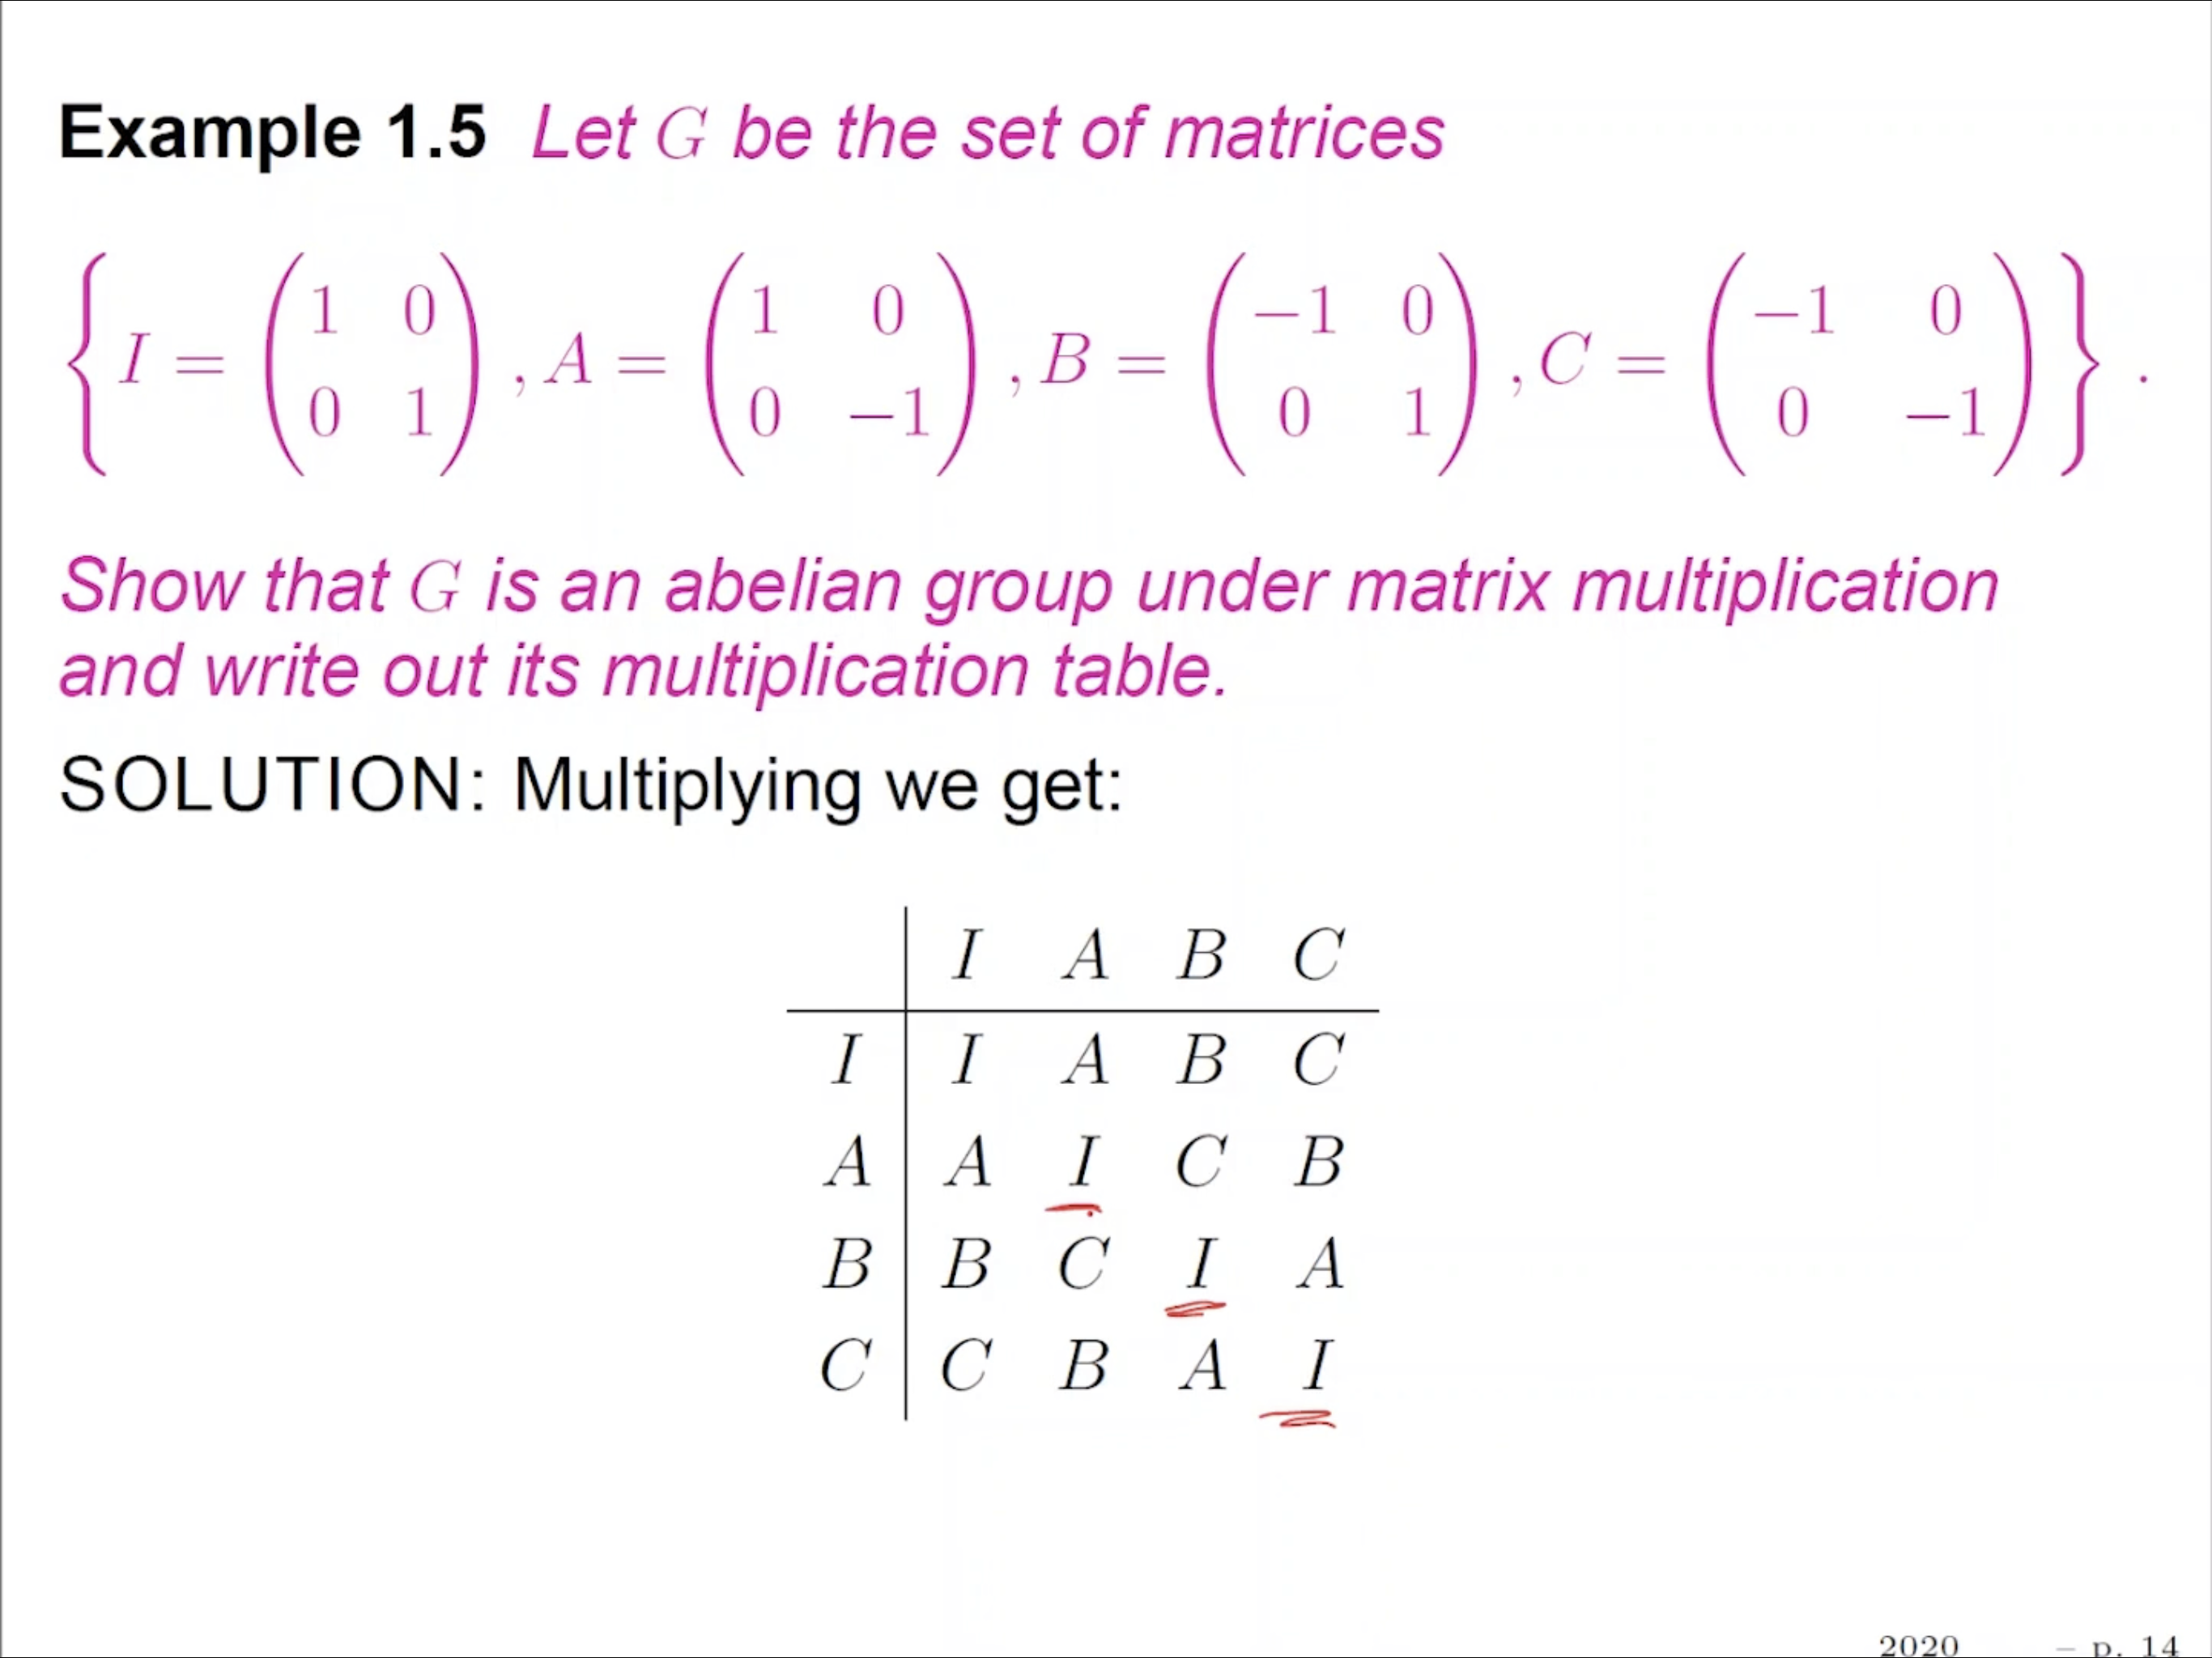
\includegraphics[scale=0.25]{assets/group_example.png}
\end{center}
\definition{Fields}{A field $(\mathbb{F}, +, \times)$ is a set $\mathbb{F}$ with two binary operations on it, addition $(+)$ and multiplication $(\times)$, where\begin{enumerate}\item $(\mathbb{F}, +)$ is an abelian gruop;\item $\mathbb{F}^* = \mathbb{F} \ \{0\}$ is an abelian group under multiplication, with $0$ being the additive identity;\item The distributive laws $a \times (b + c) = a \times b + a \times c$ and $(a + b) \times c = a \times c + b \times c$ hold.\end{enumerate}Note this satisfies the $12=5 + 5 + 2$ number laws.\\[1\baselineskip]\textsuperscript{*}It is called a `field' to resemble fields in physics; that is, a premise upon which there is rich structure and interplay.}~\\
\lemma{Interplay Between $+$ and $\times$}{Let $\mathbb{F}$ be a field and $a,b,c \in \mathbb{F}$. Then\begin{itemize}\item $a0 = 0$ (additive identity); \item $a(-b) = -(ab)$ (associativity); \item a(b-c) = ab - ac (distributive law); \item if $ab = 0$ then either $a = 0$ or $b = 0$ (proof: suppose $ab = 0$ and $a \neq 0$, then multiply both sides by $a^{-1}$ to give $0 = a^{-1}0 = a^{-1}(ab) = (a^{-1}a)b = 1b = b)$.\end{itemize}}~\\
\definition{Subgroups}{Let $(G,*)$ be a group and $H$ a non-empty subset of $G$.\\Then $H$ is a subgroup of $G$ if $H$ is a group under the restriction of $*$ to $H$.\\We write this as $H \leq G$ and say $H$ inherits the group structure from $G$.\\[1\baselineskip]\textsuperscript{*}The idea is that $H$ is just a smaller bunch of objects within $G$, the whole collection, and also has its structure and properties.}~\\
\lemma{The Subgroup Lemma}{Let $(G, *)$ be a group and $H$ and non-empty subset of $G$.\\Then $H$ is a subgroup of $G$ if and only if \begin{itemize}
  \item for all $a,b \in H$, $a * b \in H$;
  \item for all $a \in H$, $a^{-1} \in H$;
\end{itemize}These are all proved from closure and inverse of the group; associativity is inherited from $G$ and an identity exists via the inverse.\\[1\baselineskip]Note that any subgroup of an abelian group is also an abelian group.}~\\
\textbf{Examples}\begin{enumerate}
  \item Every non-trivial group $G$ has at least two subgroups: $\{e\}$ and $G$.
  \item For any integer $m$ let $m\mathbb{Z}$ be the set of all multiples of $m$. Then $(m\mathbb{Z}, +)$ is a subgroup of $(\mathbb{Z}, +)$. The converse is also true; any subgroup of $(\mathbb{Z}, +)$ is $(m\mathbb{Z}, +)$ for some $m$.
  \item Consider $C_m = <a : a^m = e>$ the cyclic group of order $m$.\\Picking any integer $k$ with $1 < k < m$ we could generate a subgroup $H_k = <a^k>$ of $C_m$ by looking at all powers of $a_k$. Clearly, the order of $H_k$ cannot be larger than $m$; it is strictly less than $m$ if and only if $k$ and $m$ have a common divisor $d > 1$.
  \item Let $n \geq 1$ be any integer. The set of invertible $n \times n$ matrices over a field $\mathbb{F}$ s a group under matrix multiplication. It is non-abelian if $n > 1$. It is called the general linear group GL$(n, \mathbb{F})$.\\They have important subgroups, such as the special linear groups SL$(n,\mathbb{R})$ and SL$(n, \mathbb{C})$ of matrices with determinant $1$, and the group of orthogonal matrices $O(n) \leq$ GL$(n, \mathbb{R})$.
\end{enumerate}\newpage
\definition{Subfields}{If $(\mathbb{F}, +, \times)$ is a field and $\mathbb{E} \subseteq \mathbb{F}$ is also a field under the same operations, then $(\mathbb{E}, +, \times)$ is a subfield of $(\mathbb{F}, +, \times)$, usually written $\mathbb{E} \leq \mathbb{F}$.}~\\
\lemma{The Subfield Lemma}{Let $\mathbb{E} \neq \{0\}$ be a non-empty subset of field $\mathbb{F}$.\\Then $\mathbb{E}$ is a subfield of $\mathbb{F}$ if and only if for all $a,b \in \mathbb{E}$ \[a + b \in \mathbb{E}, \quad -b \in \mathbb{E}, \quad a \times b \in \mathbb{E}, \quad b^{-1} \in \mathbb{E} \; \text{if} \; b \neq 0.\]Proof: The distributive laws are inherited from $\mathbb{F}$, and the rest of the proof comes from applying the subgroup lemma to $(\mathbb{E}, +)$ and $(\mathbb{E}, \times)$.}~\\
\definition{Morphisms}{Let $(G, *)$ and $(H, \circ)$ be two groups. A (group) homomorphism from $G$ to $H$ is a map $\phi : G \rightarrow H$ that respects the two operations, that is where \[\phi(a * b) = \phi(a) \circ \phi(b) \quad \text{for all} \; a,b \in G.\]A bijective homomorphism $\phi: G \rightarrow H$ is called an isomorphism; the groups are then said to be isomorphic, and are considered the same group. isomorphism is an equivalence relation.\\[1\baselineskip]\textsuperscript{*}The word `homomorphism' comes from the Ancient Greek language: homos meaning ``same'' and morphe meaning ``form'' or ``shape''.\\[1\baselineskip]\textsuperscript{**}Homomorphic maps preserve the structure of the domain group while respecting that of the codomain. The idea is if $a * b$, then under the map $\phi$, we hope that (mapped) $a$ behaves the same with (mapped) $b$ in the codomain. If so, they are homomorphic.}~\\
\textbf{Example}. Let $m \geq$ 2 be any integer. Define $\phi: (\mathbb{Z},+) \rightarrow (m\mathbb{Z},+)$ by $\phi(a) = ma$. Show that $\phi$ is an isomorphism of groups.\\
\textbf{Solution.} Firstly \[\phi(a+b)=m(a+b)=ma+mb=\phi(a)+\phi(b).\]The easiest way to show $\phi$ is a bijection is to find the inverse. But if $g \in m\mathbb{Z}$ then $g=ma$ for some $a \in \mathbb{Z}$ and clearly $\phi(a) = g$, so $\phi^{-1}(g) = a$. Thus $\phi$ is an isomorphism.\\[1\baselineskip]
\lemma{Homomorphism Lemma}{Let $(G, *)$ and $(H, \circ)$ be two groups and $\phi$ a homomorphism between them. Then \begin{itemize}\item $\phi$ maps the identity of $G$ to the identity of $H$.\item $\phi$ maps inverses to inverses, i.e. $\phi(a^{-1})=(phi(a))^{-1}$ for all $a \in G$.\item if $\phi$ is an isomorphism frmo $G$ to $H$ then $\phi^{-1}$ is an isomorphism from $H$ to $G$.\end{itemize}}~\\
\definition{Kernel and Image}{Let $\phi : G \rightarrow H$ be a group homomorphism, with $e'$ the identity of $H$.\\The kernel of $\phi$ is the set \[\text{ker}(\phi) = \{g \in G: \phi(g) = e' \}.\]It is the information lost in the map.\\The image of $\phi$ is the set \[\text{im}(\phi) = \{h \in H : h = \phi(g)\}, \; \text{for some} \; g \in G\].It is the approximation given by the map.}~\\
\lemma{Kernel and Image Lemma}{For $\phi : G \rightarrow H$ a group homomorphism, $\text{ker}(\phi) \leq G$ and $\text{im}(\phi) \leq H$.}~\\
\lemma{Isomorphism Lemma}{A homomorphism $\phi$ is one-to-one if and only if $\text{ker}(\phi) = \{e\}$, with $e$ the identity of $G$. If $\phi$ is one-to-one then $text{im}(\phi)$ is isomorphic to $G$.}~\\
\definition{Linear Representation of $G$ on $\mathbb{F}^n$}{If there exists a homomorphism $\phi : G \rightarrow$ GL$(n, \mathbb{F})$ for some $n$ and some field $\mathbb{F}$, then the group im$(\phi)$ is called a linear representation of $G$ on $\mathbb{F}^n$.\\If $\phi$ is one-to-one (so every element maps to a distinct matrix), we call the representation faithful.}~\\
\definition{Permutation Representation}{From above, in the case where $G$ is finite and $H$ is $\mathcal{S}_n$ for some $n$, then we get a permutation representation of the group $G$ as a subgroup of $S_n$.}\newpage
\definition{Vector Space}{Let $\mathbb{F}$ be a field. A vector space over the field $\mathbb{F}$ consists of an abelian group $(V, +)$ and a function from $\mathbb{F} \times V$ to $V$ called scalar multiplication and written $\alpha \vect{v}$ where \begin{enumerate} \item $\alpha(\beta \vect{v}) = (\alpha \beta)\vect{v}$ for all $\alpha, \beta \in \mathbb{F}$ and $\vect{v} \in V$. \item $1\vect{v} = \vect{v}$ for all $\vect{v} \in V$. \item $\alpha (\vect{u} + \vect{v}) = \alpha \vect{u} + \alpha \vect{v}$ for all $\alpha \in \mathbb{F}$ and $\vect{u}, \vect{v} \in V$. \item $(\alpha + \beta) \vect{u} = \alpha \vect{u} + \beta \vect{u}$ for all $\alpha, \beta \in \mathbb{F}$ and $\vect{u} \in V$.\end{enumerate}There are ten axioms here; 5 from the abelian group, closure of scalar multiplication, and four explicit ones. The $+$ in $(V, +)$ may be distinguished as vector addition.}~\\
\lemma{2.1}{Let $V$ be a vector space over field $\mathbb{F}$. For all $\vect{v}, \vect{w} \in V$ and $\lambda \in \mathbb{F}$ then \begin{itemize}
  \item $0\vect{v} = \vect{0}$ and $\lambda \vect{0} = \vect{0}$.
  \item $(-1)\vect{v} = -\vect{v}$.
  \item $\lambda \vect{v} = \vect{0}$ implies either $\lambda = 0$ or $\vect{v} = \vect{0}$.
  \item If $\lambda \vect{v} = \lambda \vect{w}$ and $\lambda \neq 0$ then $\vect{v} = \vect{w}$.
\end{itemize}}~\\
\textbf{Standard Vector Space Examples.}
\begin{enumerate}
  \item $n$-tuples.\begin{center}
    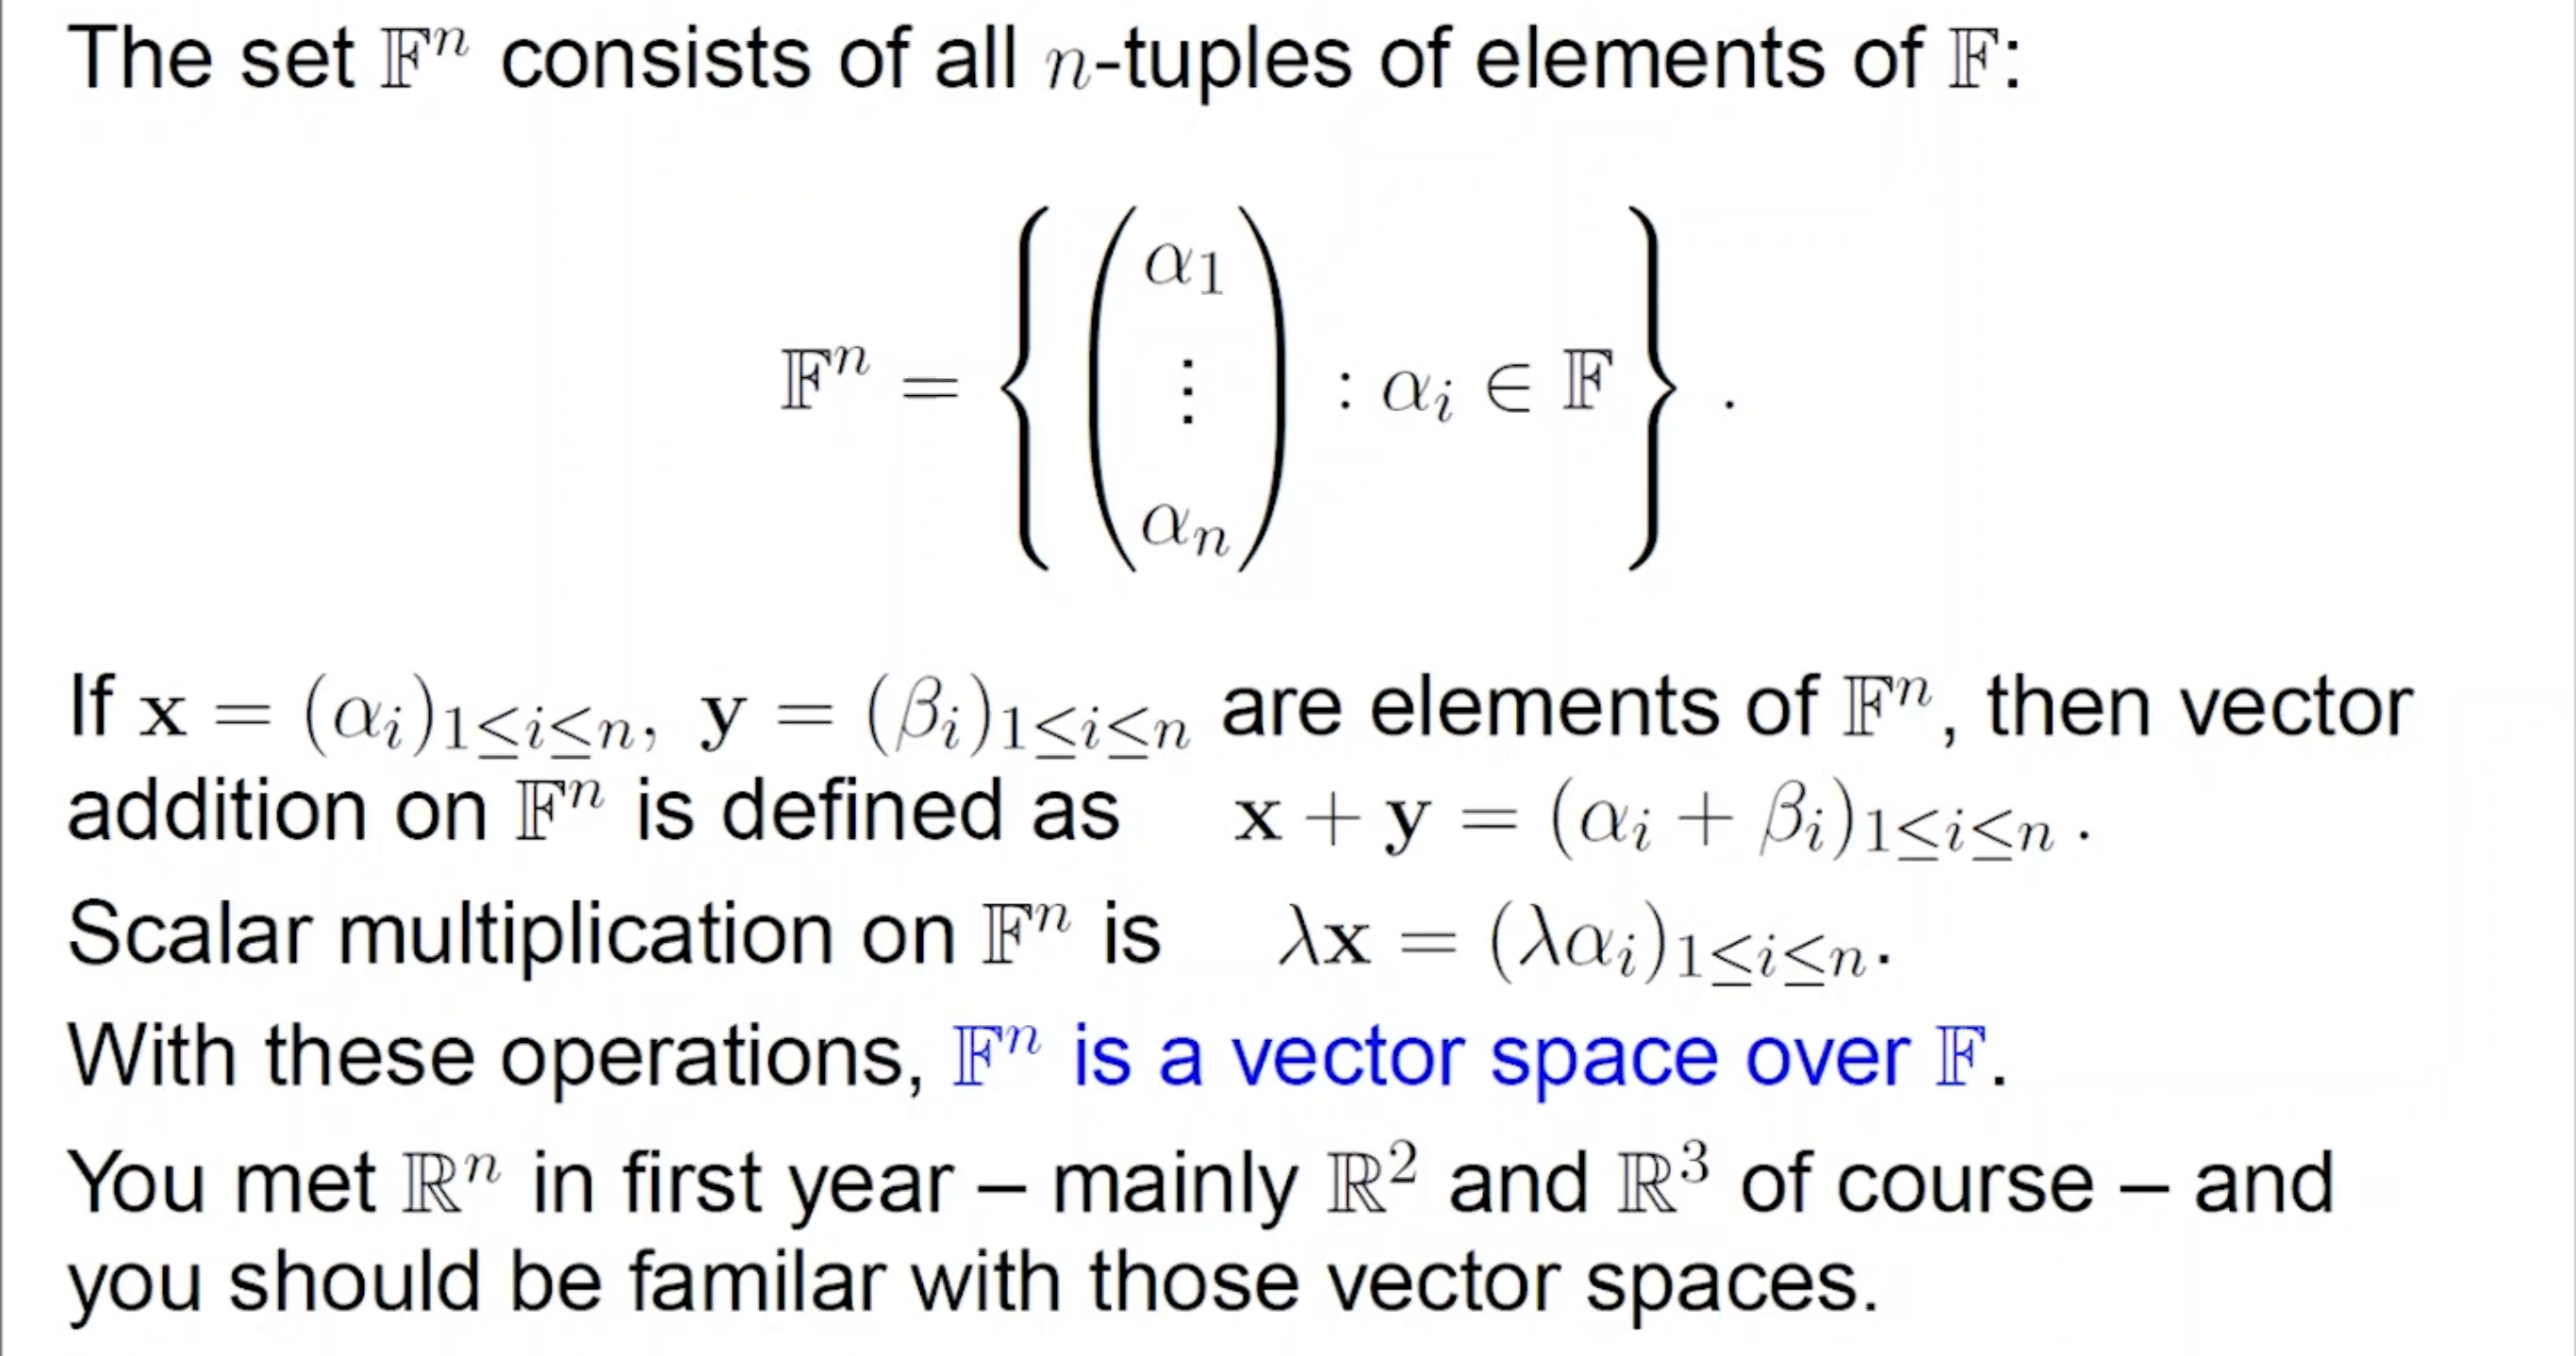
\includegraphics[scale=0.3]{assets/vector_space_eg.png}\newpage
  \end{center}
  \item Geometric Vectors.\begin{center}
    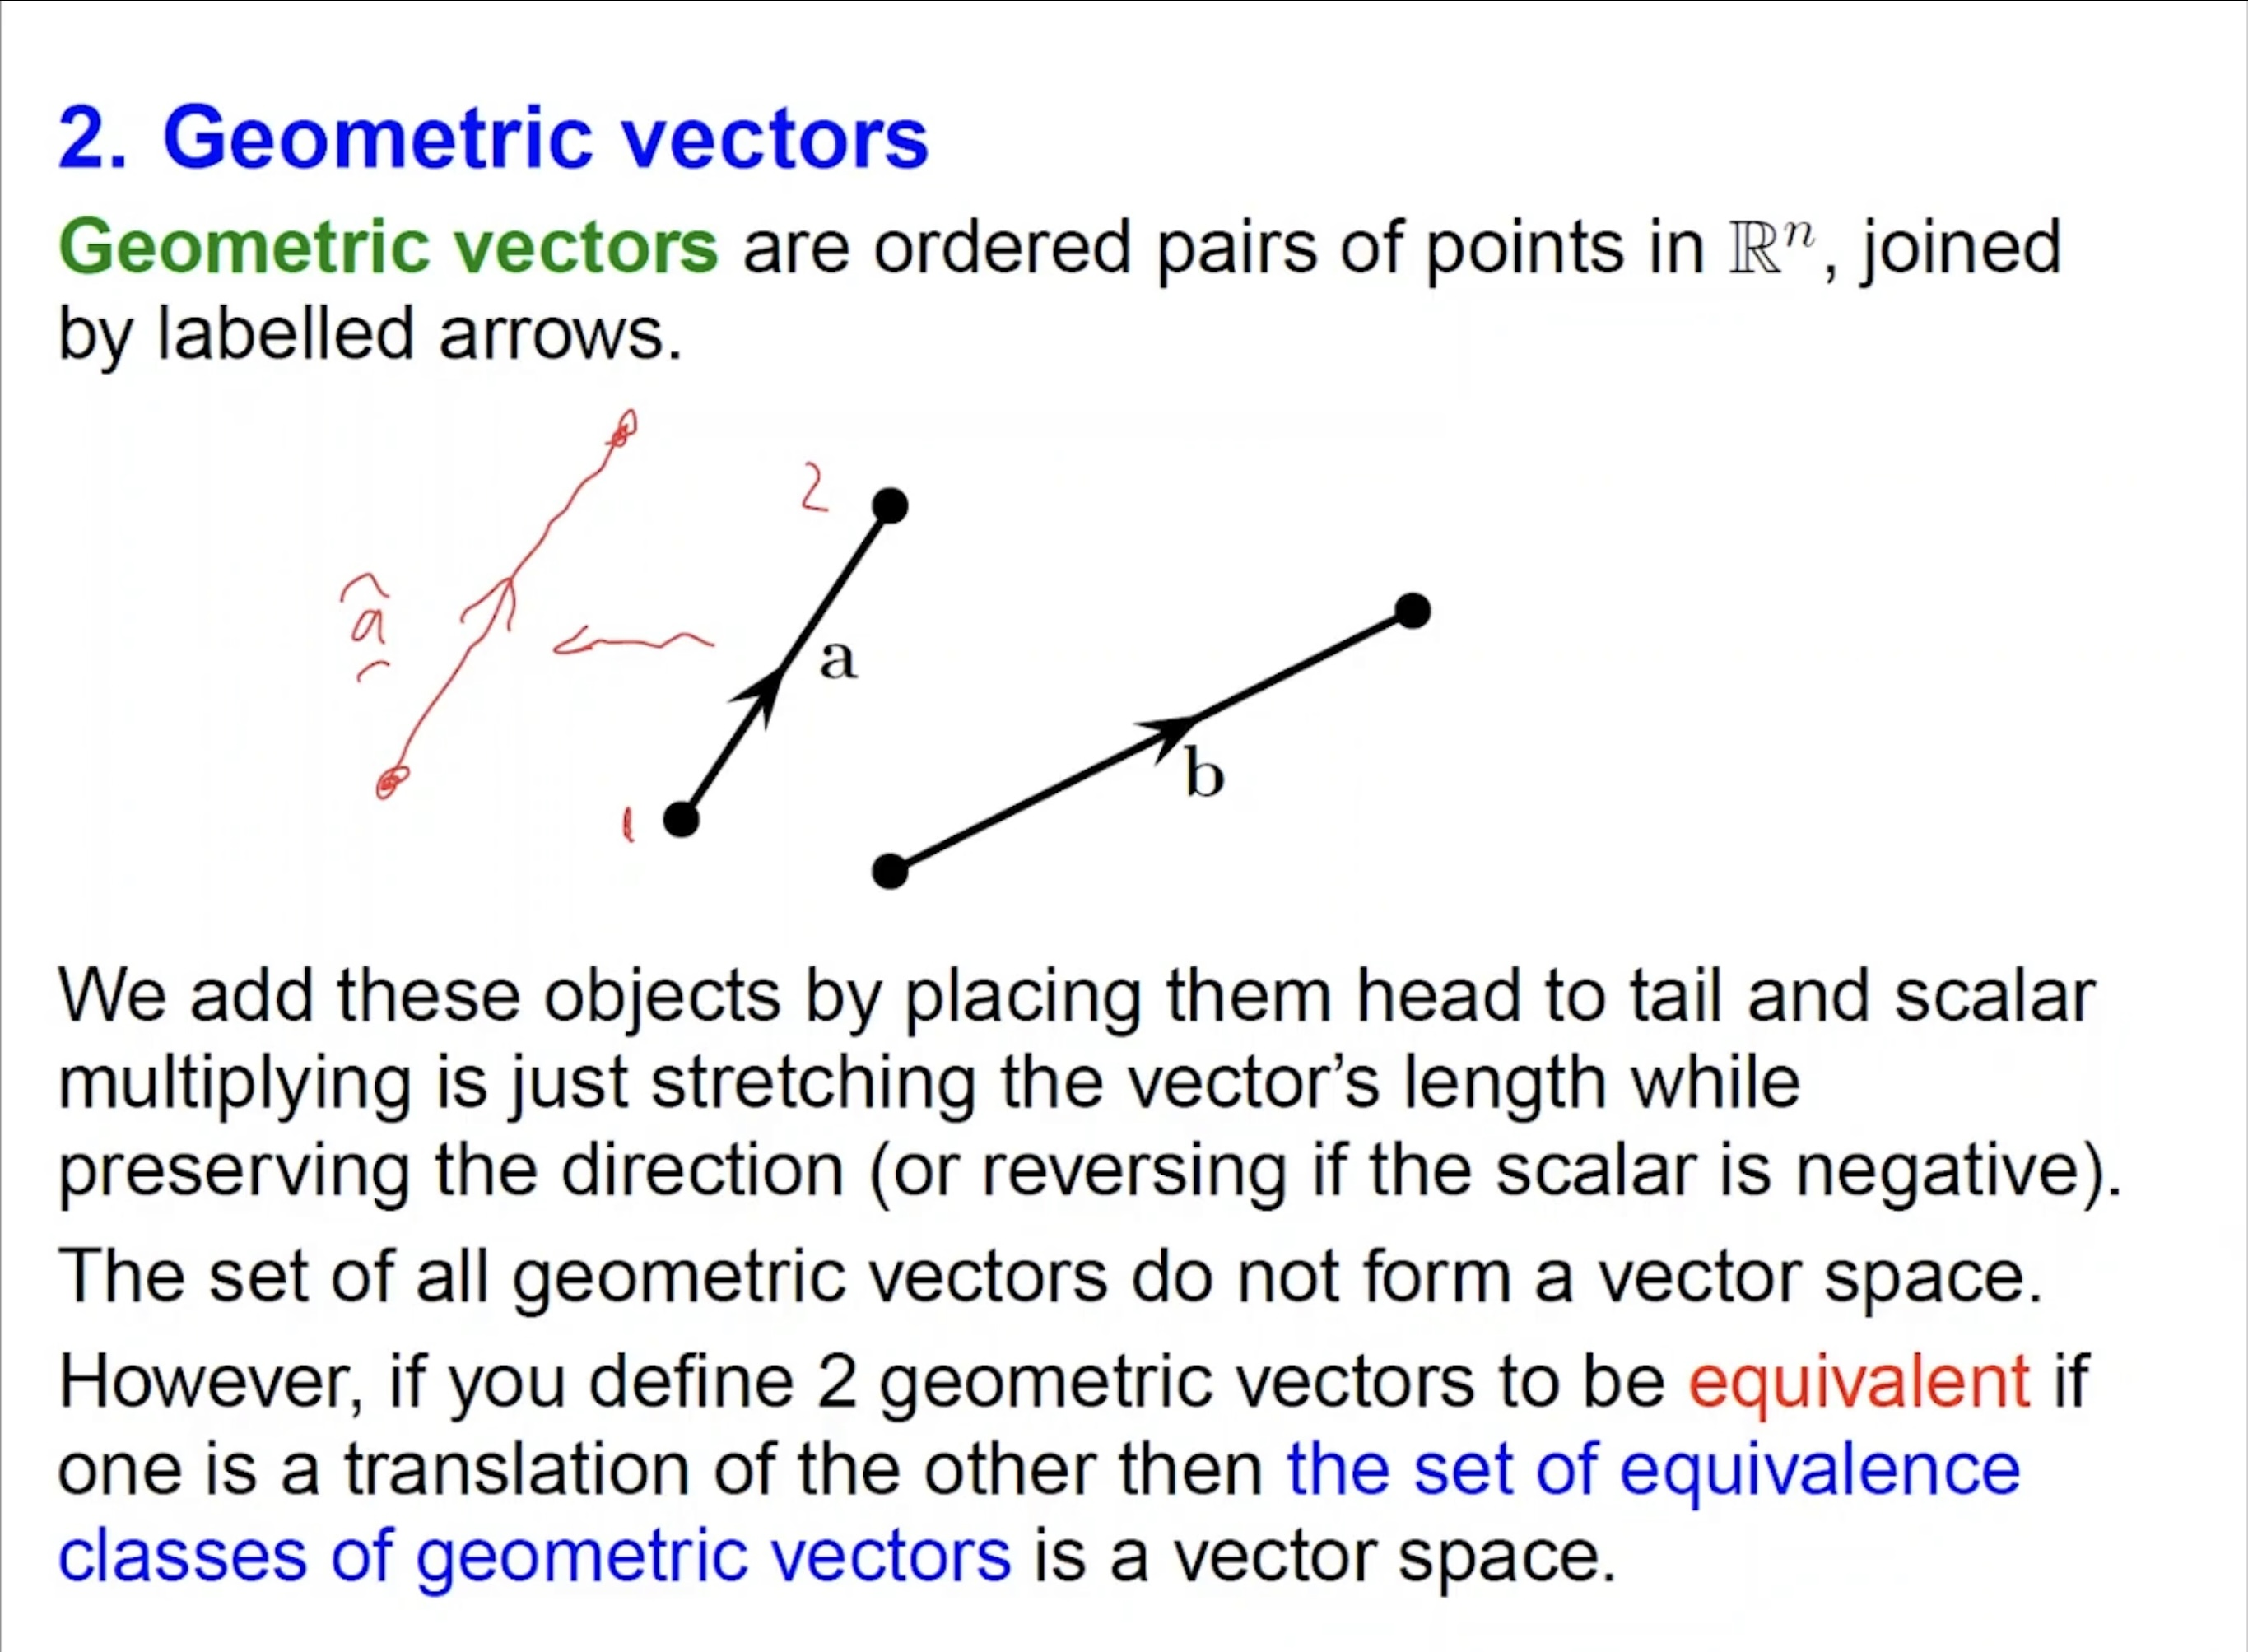
\includegraphics[scale=0.10]{assets/geometric_vecs.png}
  \end{center}
  \item Matrices.\\For any positive integers $p$ and $q$ the set $M_{p,q}(\mathbb{F})$ is the set of $p \times q$ matrices with elements from $\mathbb{F}$.\\Then $M_{p,q}(\mathbb{F})$ is a vector spsace over $\mathbb{F}$ with vector addition with the usual addition of matrices and scalar multiplication multiplying each element of the matrix.
  \item Polynomials.\\The set of all Polynomials with coefficients in $\mathbb{F}, \mathcal{P}(\mathbb{F}),$ is a vector space over $\mathbb{F}$ with \[(f+g)(x) = f(x) + g(x) \quad \text{for all} \quad x \ in \mathbb{F} \\ (\lambda f)(x) = \lambda f(x) \quad \text{for all} \quad \lambda, x \in \mathbb{F}.\]Similarly, $\mathcal{P}(F)$ (polynomials of degree $n$ or less) is a vector space over $\mathbb{F}$. Note this example shows `vector spaces' can appear abstract from actual vectors! We just need vector $+$ and $\times$.
  \item Function Spaces.\\Let $X$ be a non-empty set and $\mathbb{F}$ be a field. Then define \[\mathcal{F}[X] = \{f: X \rightarrow \mathbb{F} \}.\]The set $\mathcal{F}[X]$ is a vector space over $\mathbb{F}$ if we define \begin{itemize}\item the zero in $\mathcal{F}[X]$ to be the zero function: $x \rightarrow 0$ for all $x \in X$.
  \item $(f+g)(x) = f(x) + g(x)$ for all $x \ in X$.
  \item $(\lambda f)(x) = \lambda (f(x))$ for all $x \in X$.
  \end{itemize}
\end{enumerate}

\end{document}